% LaTex
%\documentclass[aps,twocolumn]{revtex4-1}
\documentclass[a4paper,preprint,unsortedaddress]{revtex4-1}
%\documentclass[a4paper]{article}
\usepackage{amsmath,amssymb,amsfonts,latexsym,graphicx}
\usepackage[dvips]{color}
\usepackage{indentfirst} 

% \parindent=0mm
% \textheight=23cm \textwidth=14cm
% \parskip=0mm
% \renewcommand\baselinestretch{1.2}
% \oddsidemargin30pt \evensidemargin30pt

\def\pd#1#2{\frac{\partial #1}{\partial #2}}
\renewcommand{\vec}[1]{\mbox{\boldmath \small $#1$}}
\newcommand{\concen}{C}
\setlength\parindent{2em} 
\newcommand{\recheck}[1]{{\color{red} #1}}
\newcommand{\redc}[1]{{\color{red} #1}}            
\newcommand{\vect}[1]{\textbf{\textit{#1}}}
\newcommand{\dof}{{\textrm{DOF}}}
\newcommand{\AT}{{\textrm{{AT}}}}
\newcommand{\EX}{{\textrm{EX}}}
\newcommand{\CG}{{\textrm{CG}}}
\newcommand{\HY}{{\Delta}}
\newcommand{\rdf}{{\textrm{rdf}}}
\newcommand{\thf}{{\textrm{th}}}
\newcommand{\res}{{\textrm{rep}}}
\newcommand{\ext}{{\textrm{extra}}}
\newcommand{\exc}{{\textrm{exc}}}
\newcommand{\thermo}{{\textrm{Q}}}
\newcommand{\hadress}{{\textrm{H}}}
\newcommand{\dadress}{{\textrm{D}}}


\begin{document}
%--------------------------------------------------------------------
%-----------------------------------------------------------------
\title{Chemical potential of liquids and mixtures via Adaptive Resolution Simulation}
\author{Animesh Agarwal}
\affiliation{Institute for Mathematics, Freie Universit\"at Berlin, Germany}
\author{Han Wang}
\email{han.wang@fu-berlin.de}
\affiliation{Institute for Mathematics, Freie Universit\"at Berlin, Germany}
\author{Christof Sch\"{u}tte}
\affiliation{Institute for Mathematics, Freie Universit\"at Berlin, and Zuse Institute Berlin (ZIB), Berlin, Germany}
\author{Luigi Delle Site}
\email{dellesite@fu-berlin.de}
\affiliation{Institute for Mathematics, Freie Universit\"at Berlin, Germany}


\begin{abstract}
We employ the adaptive resolution approach AdResS, in its recently developed Grand Canonical-like version (GC-AdResS) [Wang {\it et al.} Phys.Rev.X 3, 011018 (2013)], to calculate the excess chemical potential, $\mu^{ex}$, of various liquids and mixtures.
We compare our results with those obtained from full atomistic simulations using the technique of thermodynamic integration and show a satisfactory agreement. In GC-AdResS the procedure to calculate $\mu^{ex}$ corresponds to the process of standard initial equilibration of the system; this implies that, independently of the specific aim of the study, $\mu^{ex}$, for each molecular species, is automatically calculated every time a GC-AdResS simulation is performed. 
\end{abstract}

\maketitle

\section{Introduction}
The chemical potential represents an important thermodynamic information for any system, in particular for liquids, where the possibility of combining different substances for forming optimal mixtures is strictly related to knowledge of the chemical potential of each component in the mixture environment. In this perspective, molecular simulation represents a powerful tool for predicting the chemical potential of complex molecular systems. Popular, well established methodologies in Molecular Dynamics (MD) are Widom particle insertion (IPM) \cite{widom} and thermodynamic integration (TI) \cite{ti}. IPM is computationally very demanding often beyond a reasonable limit even in presence of large computational resources, but upon convergence, is rather accurate. TI is computationally convenient but specifically designed to calculate the chemical potential and thus  it may not be optimal for employing MD for studying other properties. In fact TI requires artificial modification of the atomistic interactions (see Appendix).
Recently we have suggested that the chemical potential could be calculated by employing the Adaptive Resolution Simulation method in its Grand Canonical-like formulation (GC-AdResS) \cite{prl12,jctchan,prx}.
AdResS was originally designed  to interface regions of space at different levels of molecular resolution within one simulation set up. This allows for large and efficient multiscale simulations where the high resolution region is restricted to a small portion of space and the rest of the system is at coarser level. The recent version of the method, GC-AdResS, given its theoretical framework, should automatically calculate the chemical potential during the process of initial equilibration: in this work we prove that this is indeed the case and report results for the chemical potential for various liquids and mixtures of particular relevance in (bio)-chemistry and material science. We compare our results with those from full atomistic TI and find a satisfactory agreement. This agreement allows us to conclude that every time a multiscale GC-AdResS is performed, $\mu^{ex}$ is automatically calculated for each liquid component and implicitly confirm that the basic thermodynamics of the system is well described by the method.
Below we provide the basic technical ingredients of GC-AdResS which are relevant for the calculation of the chemical potential, more specific details can be found in \cite{jctchan, prx}.
\section{From AdResS to GC-AdResS}
The original idea of AdResS is based on a simple intuitive physical principle:
\begin{itemize}
\item divide the space in three regions, one with atomistic resolution and one with coarse-grained (spherical) resolution interfaced by a smaller region with an hybrid treatment.
\item couple the molecules in the different regions through a spatial interpolation formula on the forces:
\begin{equation}
{\bf F}_{\alpha \beta}=w(X_\alpha)w(X_\beta){\bf
  F}_{\alpha\beta}^{atom}+[1-w(X_\alpha)w(X_\beta)]{\bf F}^{cg}_{\alpha\beta} 
\label{eqforce}
\end{equation}
where $\alpha$ and $\beta$ indicates two molecules, ${\bf F}^{atom}$ is the
force derived from the atomistic force field and  ${\bf F}^{cg}$
from the corresponding coarse-grained potential, $X$ is the $x$ coordinate of the center of mass of
the molecule and $w$ is an interpolating function which smoothly goes from $0$
to $1$ (or vice versa) in the interface region ($\Delta$) where the lower resolution is then
slowly transformed (according to $w$) in the high resolution (or vice versa),
as illustrated in Fig.\ref{fig1}. .  
\item In the interface region a thermodynamic force acting on the center of mass (CM) of each molecule and a locally acting thermostat are added to assure the overall thermodynamic equilibrium at a given temperature. The thermodynamic force is defined in such a way that ${\bf F}_{th}=p_{AT}+\rho_{0}\int_{\Delta}{\bf F}_{th}({\bf r})d{\bf r}=p_{CG}$, where $p_{AT}$  is the target pressure of the atomistic system (region), $p_{CG}$ is the pressure of the coarse-grained model, $\rho_{0}$ is the target molecular density of the atomistic system (region)\cite{prl12}. An additional locally acting thermostat is added to take care of the loss/gain of energy in the transition region.
\end{itemize}
\begin{figure}
\center
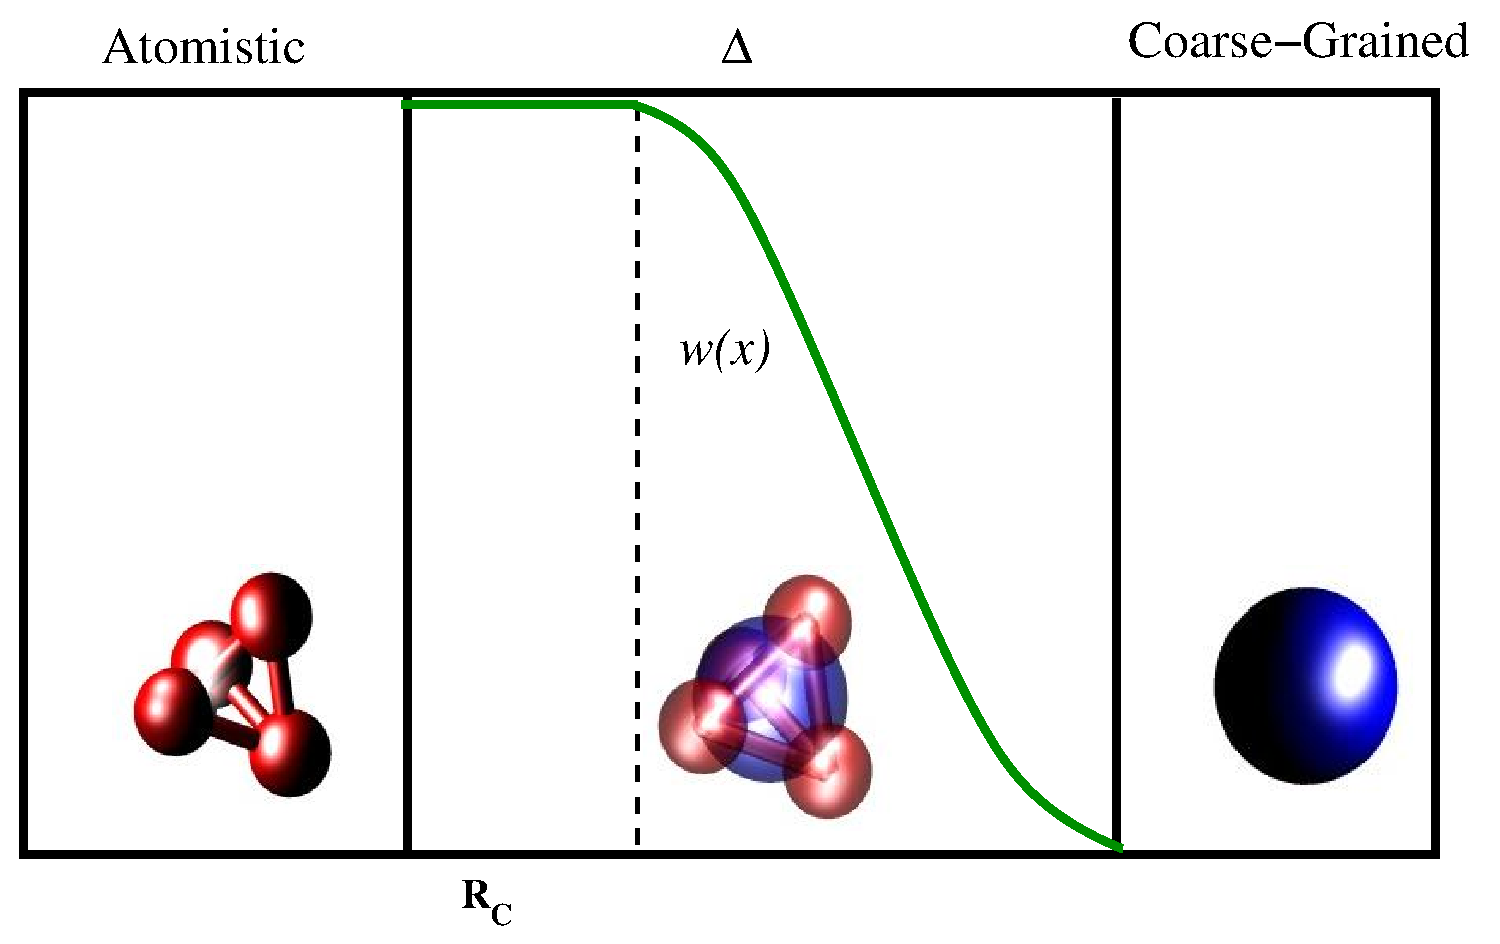
\includegraphics[width=0.475\textwidth]{adapt-schem.eps}
\caption{Pictorial representation of the adaptive box and
molecular representation. Here it is shown the case of the tetrahedral molecule used as a test case in the original development of AdResS. The region on the right,
is the low resolution region (coarse-grained), the central part is
the transition (hybrid) region $\Delta$, where the switching function
$w(x)$ (in green) is defined, and the region on the left, is the high resolution region (atomistic). It must be noticed that differently from the original AdResS, in GC-AdResS the range of definition of $w(x)$ is extended of an amount of ${\bf R}_{c}$. The extension of this additional region is equal to the cutoff radius of the atomistic interactions and $w(x)$ takes the constant value of $1$. The consequence is that molecules in the atomistic region interact with the rest of the system always and only via well defined atomistic interactions. This characteristic, in turn, allows to write an exact Hamiltonian for the atomistic region and thus treat the system in a Grand-Canonical fashion.\label{fig1}}
\end{figure} 
In \cite{prx} we have defined necessary conditions in $\Delta$ such that the spatial probability distribution of the full-atomistic reference system was reproduced up to a certain (desired) order in the atomistic region of the adaptive system. Moreover we have shown that, because of such conditions, the accuracy in the atomistic region is independent of the accuracy of the coarse-grained model, thus, in the coarse-grained region, one can use a generic liquid of spheres whose only requirement is that it has the same molecular density of the reference system.
 In the simulation set up, ${\bf F}_{th}$ is calculated via an iterative procedure as a function of the molecular density in $\Delta$. The iterative scheme consists of calculating ${\bf F}^{i+1}_{th}({\bf r})=\frac{1}{\rho_{0}\kappa_{T}}\nabla \rho^{i}({\bf r})$, ($\kappa_{T}$ the isothermal compressibility) and the force is considered converged when in $\Delta$ the target density $\rho_{0}$ is reached. As a result, ${\bf F}_{th}({\bf r})$, acting in $\Delta$, assures that there are no artificial density variations across the system, thus it allows to accurately reproduce the first order of the probability distribution in the atomistic region. Higher orders can be systematically achieved by imposing in $\Delta$ a corrective force proportional to the gradient of the corresponding higher order of the probability distribution; for example, the gradient of the CM-CM radial distribution function for the second order. Next it was proved that indeed the target Grand Canonical distribution, that is the probability distribution of a subsystem (of the size of the atomistic region in GC-AdResS) in a large full atomistic simulation is accurately reproduced. A large number of tests were performed and the reproduction by GC-AdResS of the probability distribution was numerically proved up to (at least) the third order, more than sufficient in MD simulations. Within this framework it was finally shown that the sum of work of ${\bf F}_{th}({\bf r})$ and that of the thermostat corresponds to the difference in chemical potential between the atomistic and coarse-grained resolution; this subject is treated in the next section.
\section{Calculation of $\mu$}
In Ref.\cite{prx} it has been shown that the chemical potential of the atomistic and coarse-grained resolution are related by the following formula: 
\begin{equation}
\mu_{CG}=\mu_{AT}+\omega_{th}+\omega_{Q}
\label{mu}
\end{equation}
 with $\mu_{CG}$ the chemical potential of the coarse-grained system (in GC-AdResS this corresponds to a liquid of generic spheres), $\mu_{AT}$  the chemical potential of the atomistic system, $\omega_{th}=\int_{\Delta}{\bf F}_{th}({\bf r})d{\bf r}$ the work of the thermodynamic force in the transition region, $\omega_{Q}$ the work/heat provided by the thermostat in order to slowly equilibrate the inserted/removed degrees of freedom in the transition region. $\omega_{Q}$ is composed by two parts, one, called $\omega_{extra}$, which compensates the dissipation of energy due to the change of interactions in $\Delta$, and another, $\omega_{DOF}$, which is related to the equilibration of the reinserted/removed degrees of freedom (rotational and vibrational). According to the equipartition theorem $\omega_{DOF}$ is equal to $\frac{1}{2}k_{B}T$ per degree of freedom. $\omega_{th}$ can be calculated in a straightforward way. The calculation of $\omega_{Q}$ is instead not straightforward and we have proposed to introduce an auxiliary Hamiltonian approach where the coarse-grained and atomistic potential are interpolated, and not the forces as in AdResS. Next, we impose that the Hamiltonian system must have the same thermodynamic equilibrium of the original force-based AdResS system; this is done by introducing a thermodynamic force in the auxiliary Hamiltonian approach, which, at the target temperature, keeps the density of particles across the system as in AdResS. Since in the Hamiltonian approach we have the same equilibrium of the original adaptive (and full atomistic) system  and in addition we do not need to use a thermostat, the difference between the work of the original thermodynamic force and the work of the thermodynamic force calculated in the Hamiltonian approach gives $\omega_{Q}$. Moreover we have proven numerically, for the case of liquid water, that $\omega_{Q}=\int_{\Delta}\langle w\nabla_{x} w(x)( V_{AT}-V_{CG})\rangle_{\bf r} d{\bf r}$, where $V_{AT}$ and $V_{CG}$ are the atomistic and coarse-grained potential. The result above implies that $\omega_{Q}$ can be calculated in a straightforward way during the initial equilibration within in the standard GC-AdResS code. It must be noticed that the relation we obtained for the chemical potential is the similar to that  obtained in a complementary work by Potestio {\it et al.} \cite{h-adress}. In \cite{h-adress} an Hamiltonian approach  (H-AdResS) was explored and the expression of the chemical potential was derived via an elegant thermodynamic procedure. However, H-AdResS and GC-AdResS are essentially the same up to the first order in reproducing the probability distribution in the atomistic region. It is not a surprise that the calculation of the chemical potential can be done in a very similar way; in fact the chemical potential of a system in equilibrium requires (essentially) that the density of molecules is the same across the simulation box. The differences between the two methods emerge when higher orders of the probability distribution in the atomistic region are required. However the intention of this paper is not to discuss the difference between the two methods but rather to show their capability in accurately calculating the chemical potential; a discussion about the difference between the two approaches of AdResS can be found in \cite{luigientropy}. At this point according to \eqref{mu}, if one knows $\mu_{CG}$, then  GC-AdResS can automatically provide $\mu_{AT}$. However we need to do one step more, in fact the quantity of interest is not the total chemical potential, but the excess chemical potential $\mu^{ex}_{AT}$ which corresponds to the expression of \eqref{mu} where the kinetic (ideal gas) part is subtracted. Regarding the kinetic part, one can notice that the contribution coming from the center of mass is the same for the coarse-grained and for the atomistic molecules, thus it is automatically removed in the calculation of \eqref{mu}.
The kinetic part of $\mu_{AT}$ due to the rotational and vibrational degrees of freedom corresponds in our case to $\omega_{DOF}$ and can be calculated by hand removing $\frac{1}{2}k_{B}T$ per degree of freedom. Actually this calculation is not required, in fact the technical set up of AdResS considers the removed degrees of freedom as phantom variables but thermally equilibrate them anyway \cite{simon-ch}. Thus the heat provided by the thermostat for the rotational and vibrational part is the same in the atomistic and coarse-graining molecules and is automatically removed in the difference. Finally, the calculation of $\mu^{ex}_{CG}$ can be done with standard methods, TI or IPM, which for simple spherical molecules, like those of the coarse-grained system, requires a negligible computational cost.
In conclusion, we have the final expression:
\begin{equation}
\mu^{ex}_{AT}=\mu^{ex}_{CG}-\int_{\Delta}{F}_{th}({\bf r})d{\bf r}-\int_{\Delta}\langle w\nabla_{x} w(x) (V_{AT}-V_{CG})\rangle_{\bf r} d{\bf r}
\label{finalmu}
\end{equation}
In the next section we apply this procedure to several liquids and mixtures.
\section*{Results and Discussion}
We have calculated $\mu^{ex}$ for different liquids and mixtures, choosing cases which are representative of a large class of systems. Hydrophobic solvation in methane/water and in ethane/water mixtures, hydrophilic solvation in urea/water, a balance of both in water/tert-Butyl alcohol (TBA) mixture, other liquids, e.g. pure methanol and DMSO (and their mixtures with water), non aqueous mixtures in TBA/DMSO and alkane liquids such as methane, ethane and propane. Moreover, systems as water/urea are commonly used as cosolvent of biological molecules \cite{nico-debashish} while systems as tert-Butyl alcohol/water play a key role in modern technology \cite{irata}, thus they are of high interest {\it per se}. All technical details of each simulation are presented in the Appendix.
Results are reported in Table \ref{table} where the comparison with values obtained using full atomistic TI and available experiments, at the same concentrations, of our calculation is made; in our previous work we have already shown that value of the chemical potential of liquid water obtained with IPM is well reproduced by GC-AdResS, however the computational cost of IMP was very large, thus we do not consider calculations done with IPM in this paper. 
The agreement with full atomistic TI simulations is satisfactory in all cases, and thus it proves the solidity of GC-AdResS in describing the essential thermodynamics of a large class of systems.
We also compare the obtained values with those available in literature \cite{vang,nico}. Although the concentration of the minor component in the mixtures that we consider, is higher than the concentrations considered in Refs.\cite{vang,nico}, we are anyway in the very dilute regime and thus the chemical potential should not change in a significant way; we have verified  such a supposed consistency. 
The chemical potential of $i$-th liquid's component in a mixture is calculated as:
\begin{equation}
\mu^{ex,i}_{AT}=\mu^{ex,i}_{CG}-\int_{\Delta}{F}^{i}_{th}({\bf r})d{\bf r}-\int_{\Delta}\langle w\nabla_{x_{i}} w(x)(V_{AT}-V_{CG})\rangle_{\bf r}d{\bf r}
\label{icomp}
\end{equation}
where ${F}^{i}_{th}(x)$ is the thermodynamic force applied to the molecules of the $i$-th component; this assures that, at the given concentration, the density of molecules of species $i$, in the transition region, is equivalent to the density of the same liquid's component in a reference full atomistic simulation. $\nabla_{x_{i}} w(x)$ is the gradient along $x$ (in a rectangular box) applied to the switching function $w(x)$ in the center of mass of molecules of component $i$. 
\begin{table}[htpb]
\begin{center}
%\begin{tabular}{ccccc}
\begin{tabular}{ccccc}
\hline \hline
 Liquid component & Mole fraction of solute & GC-AdResS & TI & Experiment \\
\hline
water    & -- & -22.8 $\pm$ 0.2  & -22.1 $\pm$ 0.3 & -23.5 \cite{florian} \\
methane  & -- & -4.6 $\pm$ 0.1  & -5.2 $\pm$ 0.1 & -- \\
ethane   & -- & -8.2 $\pm$ 0.3  &  -8.8 $\pm$ 0.1 & -- \\
propane  & -- & -8.5 $\pm$ 0.1 & -9.5 $\pm$ 0.2 & -- \\
methanol  & -- & -20.1 $\pm$ 0.1 & -20.6 $\pm$ 0.4 & -20.5 \cite{vang}  \\
DMSO & -- & -32.2 $\pm$ 0.3 & -34.7 $\pm$ 0.7 & -32.2 \cite{dmso}  \\
methanol in methanol/water mixture & 0.01 & -18.1 $\pm$ 0.2 & -19.7 $\pm$ 0.2 & -- \\
methane in methane/water mixture & 0.006 & 9.1 $\pm$ 0.1  & 8.5 $\pm$ 0.2 & -- \\
urea in urea/water mixture & 0.02 & -56.1 $\pm$ 0.6 & -58.2 $\pm$ 0.5 & -57.8 $\pm$ 2.5 \cite{urea} \\
ethane in ethane/water mixture & 0.006 & 7.2 $\pm$ 0.2 & 7.4 $\pm$ 0.3 & -- \\ 
TBA in water/TBA mixture & 0.02 & -20.5 $\pm$ 0.6 & -21.4 $\pm$ 0.5 & -- \\
DMSO in DMSO/water mixture & 0.01 & -31.4 $\pm$ 0.5 & -33.2 $\pm$ 0.3 & -- \\
TBA in TBA/DMSO mixture & 0.02 & -24.8 $\pm$ 0.4 & -24.0 $\pm$ 0.5 & -- \\
\hline \hline
\end{tabular}
\caption{The excess chemical potential of different liquids and mixtures in $kJ/mol$ calculated from GC-AdResS and TI of full atomistic simulations. Experimental values for systems at the same concentrations used in simulation are also reported for comparison. For pure systems (water and methanol) we compare our values with those obtained in literature using the same force field and computational code. For mixtures, most of the values from literature (simulation and experiments) are available at lower concentrations (see Refs.\cite{vang,nico}); however since we are always in a very dilute regime the chemical potential does not change significantly; we have verified that such consistency holds. Note that the chemical potential of water in dilute mixtures is the same of pure water and is not reported above.
}
\label{table}
\end{center}
\end{table}

\begin{figure}
\center
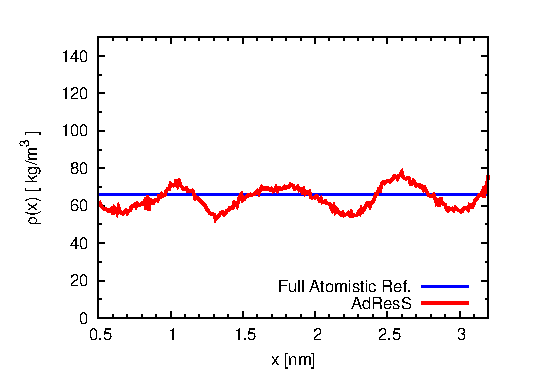
\includegraphics[width=0.475\textwidth]{alcohol_rho.eps}\\
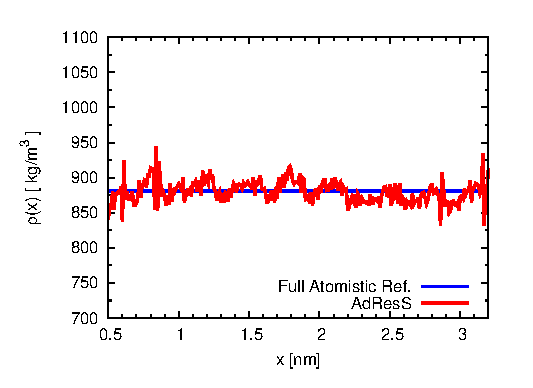
\includegraphics[width=0.475\textwidth]{water_rho.eps}
\caption{Top: Molecular density profile in $\Delta$ for TBA/water mixture; bottom, the same plot for water. Among all the systems considered, in this case the action of the thermodynamic force and that of the thermostat leads to the largest deviation from the reference all atomistic average density; however even in this case the discrepancy is negligible.\label{urea-TBA}}
\end{figure}
\begin{figure}
\center
\includegraphics[width=0.475\textwidth]{alcohol-alcohol.eps}\\
\includegraphics[width=0.475\textwidth]{alcohol-water.eps}\\
\includegraphics[width=0.475\textwidth]{water-water.eps}
\caption{Top: TBA-TBA radial distribution function; middle: the same plot for TBA-water; bottom: for water-water. The $g(r)$ is calculated only in the atomistic region.  Molecules located beyond a distance equal to the interactions' cut off, $0.9 nm$, are not considered since would include hybrid and coarse-grained molecules. \label{gr}}
\end{figure} 
In essence, according to the results obtained, GC-AdResS allows an on-the-fly determination of $\mu^{ex}$ of each component of a liquid, whenever a simulation is performed, without extra computational costs.
Moreover, Fig.\ref{urea-TBA} shows the action of the thermodynamic force and of the thermostat in the transition region $\Delta$ for TBA-water; the molecular density is sufficiently close to that of reference (the largest difference is below $20\%$ and the average difference is below $10\%$), and thus it assures that in the atomistic region there are no (significant) artificial effects on the molecular density due to the perturbation represented by the interpolation of forces in $\Delta$. In Fig.\ref{gr} we report various radial distribution functions for TBA-water in the atomistic region of the adaptive set up. The agreement with data from a full atomistic simulation is highly satisfactory. Moreover, it must be underlined that, on purpose, we have chosen extreme technical conditions, that is, a very small atomistic and coarse-grained region ($0.5 nm$) and a relatively large transition region ($2.7 nm$). Even in these conditions we prove that local properties as those of Fig.\ref{urea-TBA} and Fig.\ref{gr}, together with a relevant thermodynamics quantity as $\mu^{ex}$ are well reproduced.
This example shows the key features of GC-AdResS, that is, a multiscale simulation where the chemical potential of each component is obtained without extra computational costs and with high accuracy in a simulation where other properties are also calculated with high accuracy. It must be also noticed that the system corresponding to the figures is, among all the system considered, the case where the action of the thermodynamic force and of the thermostat produces the less accurate agreement with the reference data.
\section{Current computational convenience: a critical appraisal}
The natural question arising from the discussion above is whether or not GC-AdResS is a more convenient technical tool for calculating $\mu^{ex}$ compared to TI.
Currently the answer is negative although the current work is the first step towards a potentially positive answer for the future. In fact, the fastest version of AdResS is implemented in the GROMACS code \cite{gromacs}; using the Gromacs version 4.5.1 a speedup of a factor four with respected to full atomistic simulations has been reported for aqueous mixtures~\cite{debashish1,nico-debashish}. In this case GC-AdResS was more convenient than TI because in one simulation one could obtain the chemical potential of each liquid component and at the same time calculate structural properties (e.g. radial distribution functions). However in the successive version of GROMACS 4.6.1 the performance of atomistic simulations (above all of SPC/E water) has been highly improved while the corresponding implementation of AdResS is not optimized yet. At the current state, AdResS can only assure a speed up factor between 1.5 and 1.9 for large systems (30000 molecules) compared to full atomistic simulations without SPC/E water. As a consequence for the calculation of $\mu^{ex}$, TI is computationally less demanding than AdResS. Another point that must be considered (in perspective) for a fair comparison between TI and GC-AdResS, is the following: even if AdResS is optimized, in any code, TI has the advantage that one can use one single molecule in the simulation box to mimic the minor component of a mixture. In our case, instead, we must treat, technically speaking, a true mixture with a certain number of molecules of the minor component immersed in the liquid of the major component. Thus, at low concentrations, GC-AdResS simulations require larger systems than those required by TI, moreover, because of the low density of the minor component, the convergence of the corresponding thermodynamic force requires long simulations. 
Thus, for very dilute systems, if one is interested only in the chemical potential, TI shall be preferred to GC-AdResS, however if the interest goes beyond the calculation of the chemical potential, (e.g. radial distribution functions) then (optimized) GC-AdResS would still be more convenient.
When the concentration becomes higher, GC-AdResS may become preferable for both tasks: general properties of the mixture and chemical potential, not only because in this case one requires larger systems, but also because the convergence of the thermodynamic force of the minor component is much faster. Moreover, we would have the flexibility of calculating the chemical potential
of both components in one simulation run, whereas in TI, one needs to run two separate simulations in order to get the chemical potential of both components.
However, at the current state, the technical aspects of code optimization must be reported and we must make clear that the aim of this work is to show that  the automatic calculation of $\mu^{ex}$, independently from the simulation code in which is implemented and its computational cost, is a ``conceptual'' feature of GC-AdResS.
  
\section*{Conclusion} 
We have shown the accuracy of GC-AdResS in calculating the excess chemical potential for a representative class of complex liquids and mixtures. 
For any system, the initial equilibration process, that is the determination of the thermodynamic force, automatically delivers the chemical potential. The only additional calculation required is that of $\mu^{ex}_{CG}$ which implies the use of IPM or TI, but for a liquid of simple spheres, thus computationally negligible.  
The essential message is that GC-AdResS would be, {\it per se}, a reliable multiscale technique to calculate the chemical potential and, in perspective, upon computational/technical optimization it may become an efficient tool for calculating $\mu^{ex}$ compared to current techniques in MD such as TI. 

\section*{Acknowledgments}
This work was supported by the Deutsche Forschungsgemeinschaft (DFG) with the Heisenberg grant provided to L.D.S (grant code DE 1140/5-1) and with its associate DFG grants for A.G.(grant code DE 1140/7-1) and for H.W. (grant code DE 1140/4-2).H.W.~and C.S.~thank the financial support by DFG research center MATHEON.

\section*{Appendix I}
The potential energy function and the force field parameters for all the molecules
were taken from GROMOS53A6 parameter set. Liquid water was described by the SPC
model~\cite{spc}, methanol was described by the model developed by Walser et al~\cite{walser},
urea by the model described in~\cite{urea}, tert-butyl alcohol by the parameter set of~\cite{tba}
and DMSO was described by the model given by Geerke et.al.~\cite{dmso1}. For liquid methanol simulations, 
GROMOS43A1 parameter set was used, as it was shown to be more accurate for calculating excess free energy of 
solvation of methanol in methanol~\cite{vang}. 

In all the AdResS simulations, 30 iterations were performed to obtain a 
converged thermodynamic force and a flat density profile. Each iteration consisted 
of 200 ps of equilibration which was followed by 200 ps of data collection. 
The simulations were performed at NVT conditions where the temperature was kept constant 
at 298 K. Simulations of liquid methane and ethane were performed at
111.66 K and 184.52 K respectively. To obtain the chemical potential of coarse-grained component, 
insertion particle method was used, where a trajectory of 8 ns was obtained and the coordinates were written
after every 0.4 ps. The insertions of the molecule were performed 4,000,000 times in each 
frame at random locations and with random orientations of the molecule. The chemical potential value and
the error were calculated by taking the average and standard deviation of the last ten iterations. 

The excess chemical potential of the solute or the excess free energy of solvation was calculated using the 
thermodynamic integration (TI) approach. In the thermodynamic integration, the 
interaction of solute with the rest of the molecules in the systems is a function 
of a coupling parameter $\lambda$, which indicates a level of change taken place between states
A and B. The interactions are switched off as $\lambda$ is 
continuously decreased in the stepwise manner. Simulations conducted at different values of 
$\lambda$ allow to plot a $\frac{\partial H}{\partial \lambda}$ curve, from which 
$\mu^{excess}$ is derived \cite{mu}. 
\begin{equation}
 \mu_{iB} - \mu_{iA} = \int_{0}^{1} \left \langle \frac{\partial H}{\partial \lambda} \right \rangle_{\lambda} d\lambda 
\end{equation}
where $U_{i}$ is the interaction energy of particle $i$ with the remaining particles and $\langle . \rangle$
denotes the canonical (NVT) or isobaric-isothermal (NPT) ensemble average. We computed the excess 
free energy using a two-stage approach as described in~\cite{mobley}, first coupling van der Waals interactions to transform the 
non-interacting molecule into a partially-interacting uncharged molecule, then coupling Coulomb
interactions from an uncharged interacting molecule to fully-interacting molecule. The resulting 
free energy $\Delta G_{final}$ is the sum of $\Delta G$ values obtained from the two procedures,
\begin{equation}
 \Delta G_{final} = \Delta G_{ele} + \Delta G_{vdw}
\end{equation}
where $\Delta G_{ele}$ is the free energy change associated with introducing the van der Waals interactions and 
$\Delta G_{vdw}$ is the free energy change associated with introducing Coulomb interactions. 
We evaluated the above integral for 21 values of $\lambda$ (evenly spaced between 0 and 1) in both the procedures.
At each value of $\lambda$, first a steepest descent energy minimization was performed followed 
by 200 ps of NPT equilibration and 400 ps of data collection under constant volume and temperature
conditions, in accordance with AdResS simulations. 
During the van der Waals coupling, soft-core interactions were used with soft-core parameters $\alpha_{LJ} = 0.5$, 
$\sigma = 0.3$ and the power of $\lambda$ in soft-core equation was taken as $1$. Free energy estimates and the errors
were calculated through Bennet's acceptance ratio method (BAR)~\cite{bar}. 
For both the AdResS and full-atom simulations, the system size was kept same. Below is a table 
with number of solute molecules, solvent molecules, system dimensions, size of hybrid and atomistic region (in AdResS simulations)
for each system studied. 
\begin{table}[!ht]
\begin{center}
\begin{tabular}{ccccc}
\hline \hline
 System & $N_{solute}$ & $N_{solvent}$ & System size ($nm^{3}$) &  AT + HY region ($nm^{3}$)  \\
\hline
water    & --- & 13824 & $29.9 \times 3.7 \times 3.7$ & $6.7 \times 3.7 \times 3.7$ \\
methane & --- & 2000 & $9.0 \times  3.7 \times 3.6$ & $6.0 \times 3.7 \times 3.6$ \\
ethane & --- & 2000 & $12.0 \times 3.9 \times 3.7$ & $7.0 \times 3.9 \times 3.7$ \\
propane & --- & 1433 & $10.0 \times 4.5 \times 4.5$ & $7.0 \times 4.5 \times 4.5$ \\
methanol & --- & 3200 & $9.6 \times 4.8 \times 4.8$ & $6.8 \times 4.8 \times 4.8$ \\
DMSO & --- & 1500 & $15.0 \times 3.6 \times 3.3$ &  $7.0 \times 3.6 \times 3.3$ \\
methanol/water mixture & 40 & 3960 & $9.2 \times 3.7 \times 3.7$ & $6.5 \times 3.7 \times 3.7$ \\
methane/water mixture & 40  & 6960 & $10.0 \times 4.8 \times 4.7$ & $6.5 \times 4.8 \times 4.7$ \\
urea/water mixture & 50 & 2500 & $9.7 \times 2.9 \times 2.8$ & $6.8 \times 2.9 \times 2.8$ \\
ethane/water mixture & 40 & 6960 & $10.0 \times 4.7 \times 4.6$ & $6.5 \times 4.7 \times 4.6$ \\ 
TBA/water mixture & 80 & 4400 & $10 \times 3.9 \times 3.8$ & $6.5 \times 3.9 \times 3.8$  \\
DMSO/water mixture & 50 & 4950 & $12.0 \times 4.0 \times 3.3$ & $7.0 \times 4.0 \times 3.3$ \\
TBA/DMSO mixture & 80 & 4400 & $10.0 \times 7.3 \times 7.2$ &  $7.0 \times 7.3 \times 7.2$ \\
\hline \hline
\end{tabular}
\caption{Summary of AdResS and full-atom simulations.}
\label{table2}
\end{center}
\end{table}

In all the simulations, a leap-frog stochastic dynamics integrator with a time step
of 2 fs and an inverse friction coefficient of 0.1 ps was used. All bond-lengths were constrained using the LINCS 
algorithm. In AdResS simulations, it was 
seen that the excess chemical potential values converge after a specific cut-off radius value. Hence, a different 
cut-off radius was used for different simulations in order to obtain a converged value. The full-atom simulations 
were performed using the same cut-off value to have a fair comparison. For liquid water, methanol/water, methane/water, ethane/water
and TBA/water systems, a cut-off radius of 0.9 nm was used for van der Waals and Coulomb interactions, while for rest 
of the systems, a cut-off radius of 1.4 nm was used. Electrostatic 
interactions beyond the cut-off radius were calculated using the reaction-field term \cite{rf} with a dielectric 
permittivity of 54 for urea in SPC water \cite{urea}, 64.8 for TBA in SPC water \cite{tba}, 61 for other solutes in SPC
water, 19 for methanol and 46 for DMSO as the solvent \cite{vang}. 


\section*{Appendix II: The deriviation of the $w_{extra}$}

We consider the potential interpolation of the system:
\begin{align}
  V =
  \sum_{i<j} w(\vect r_i) w(\vect r_j)
  V^\AT_{i,j}
  +
  \sum_{i<j}[1- w(\vect r_i) w(\vect r_j)]
  V^\CG_{i,j},
\end{align}
where  $\vect r_i$ denotes
the center-of-mass (COM) position of the molecule with index $i$.
$V^\AT_{i,j}$ and $V^\CG_{i,j}$ are the atomistic and coarse-grained potential energy between molecule $i$ and $j$, respectively.
Being more precisely, they are
\begin{align}
  V^\AT_{i,j} =
  \sum_{\alpha\in i}\sum_{\beta\in j} V^\AT(\vect r_\alpha - \vect r_\beta),\quad
  V^\CG_{i,j} =
  V^\CG(\vect r_i - \vect r_j).
\end{align}
where index $\alpha$ and $\beta$ denotes the atom position of the corresponding molecule.
The center of mass of the molecule can be calculated by
\begin{align}
  \vect r_i = \sum_{\alpha\in i} \frac{m_\alpha}{\sum_{\alpha\in i} m_\alpha} \vect r_\alpha,
\end{align}
where $m_\alpha$ is the mass of atom $\alpha$.
The
corresponding intermolecular force is given by
\begin{align}\label{eqn:interpol-f}
  \vect F_{i,j} =
  w(\vect r_i) w(\vect r_j)
  \vect F^\AT_{i,j}
  +
  [1- w(\vect r_i) w(\vect r_j)]
  \vect F_{i,j}^\CG
  -
  \nabla w(\vect r_i) w(\vect r_j)
  (V^\AT_{i,j} - V^\CG_{i,j})
\end{align}
We define the force of changing representation:
\begin{align}\label{eqn:frep}
  \vect F_{\res,i} = 
  \sum_j \nabla w(\vect r_i) w(\vect r_j)
  (V^\AT_{i,j} - V^\CG_{i,j})
\end{align}
An important fact is that the force of changing representation is not
symmetric w.r.t molecule $\alpha$ and $\beta$, therefore, the Newton's
action-reaction law (momentum conservation) does not hold anymore for
the potential interpolation approach. On the other hand, the force
interpolation scheme does not preserve
energy, while the potential interpolation
approach has the advantage of energy conservation. In sum, both the
force and potential interpolation approaches do not hold all physical
conservation laws, because the hybrid region is artificially
designed. Therefore, we will take the advantage of both the method and
develop the thermodynamic relation (between the atomistic and
coarse-grained resolutions)  for them at the same time.\\

We use the same notation as in our previous work~\cite{prx}.
The thermodynamic variables for the atomistic and coarse-grained regions
are denoted by $(N_1, V_1, T)$ and $(N_3, V_3, T)$, respectively.
We assume that the hybrid region is an infinitely thin filter that allows
changing of resolution when a molecule passes through it. Therefore, we
reasonably assumes that
\begin{align}
  V &= V_1 + V_3\\
  N &= N_1 + N_3
\end{align}
where $V$ and $N$ are the whole system volume and total number of
molecules in the system, respectively. In this work, we adopt the same
assumptions as those listed in Sec.III.C of Ref.~\cite{prx},
i.e. the system is under the thermodynamic limit, and is short-range
correlated. When the thermodynamic force for both approaches are calculated
(denoted by $\vect F_\thf$ and $\vect F^\hadress_\thf$, respectively.
We use the superscript H to indicate that the thermodynamic force is of the
potential interpolation AdResS),
the flat density profile is enforce to the system:
\begin{align}
  \rho_\HY &= \rho_\AT = \rho_\CG = \rho_0\\
  \rho_\HY^\hadress &= \rho_\AT = \rho_\CG = \rho_0
\end{align}
Where $\rho_0$ is the equilibrium number density of the system defined by $\rho_0 = N/V$.
The thermodynamic force in force interpolation scheme provides the
balance of the grand potential~\cite{prl12}, or equivalently
\begin{align}\label{eqn:peq}
  p_\AT = p_\CG - \rho_0 \,\omega_\thf 
\end{align}
where $p$ denotes the pressure, and $ \omega_\thf$ denotes the
integral of the thermodynamic force. \\

Since the existence of the force of changing representation breaks the
Newton's action-reaction law, the pressure relation between the AT and CG
resolution~\eqref{eqn:peq} does not hold anymore for the potential interpolation,
and should be derived again.
Now assume, for simplicity, the system only changes resolution in $x$ direction.
We impose an infinitesimal increment of the volume $\Delta V$ to the
AT region, and the same decrement of the volume $-\Delta V$ of the CG
region.  The volume of the hybrid region is kept the invariant,
so it is a ``piston''
moves toward the CG region by $\Delta L$,
where we assume $\Delta V = \Delta L\cdot S$, where $S$ is the
cutting surface area.
Here we talk about the infinitely small displacement  $\Delta L$
in the sense that it is even much smaller than the size of the
hybrid region. This is achievable by taking the limit of $\Delta L\rightarrow 0$,
while keeping the system size fixed.
Please also notice the displacement of the molecules are infinitely small,
so one can reasonably assume
the resolution of molecules remains the same under displacement $\Delta L$.
Therefore, the change of the free energy of the system is
\begin{align}\nonumber
  \Delta A \approx&\,
  A_\AT(N_1, V_1+\Delta V, T) -
  A_\AT(N_1, V_1, T)
  +
  A_\CG(N_3, V_3-\Delta V, T) -
  A_\CG(N_3, V_3, T)\\\label{eqn:apptmp3}
  &+
  \int d r\, \rho_0 S\cdot \Delta L\cdot
  \vect F^\hadress_\thf(r)
  -
  \int d r\, \rho_0 S\cdot \Delta L\cdot
  \big\langle \vect F_\res(r)\big\rangle
\end{align}
where $A_\AT$ and $A_\CG$ are the free energy of the AT and CG region, respectively.
$N_1$ and $N_3$ are the number of molecules in the AT and CG region, and
$V_1$ and $V_3$ are the volumn in the AT and CG region, respectively. $T$ is the temperature
of the system.
The last term comes from the work done on the piston. It is composed by
two parts, the fist is the work done by the thermodynamic force, and the
second is due to 
the force of changing representation, which does not vanish due to the break of the Newton's
action-reaction law. The fist and second part of Eq.~\eqref{eqn:interpol-f}
do not contribute, because they obey the Newton's action-reaction law, so
their works cancel as long as the transition region move infinitesimally toward one direction.
The notation $\langle\cdot\rangle$ in Eq.~\eqref{eqn:apptmp3} denotes the ensemble averge.
It is straightforward to show that 
\begin{align}\label{eqn:peq-d}
  \Delta A \approx
  -p_\AT\Delta V + p_\CG\Delta V -
  \rho_0 \Delta V (\omega_\thf^\hadress - \omega_\res), 
\end{align}
where $w_\thf^\hadress$ is the integral of the potential interpolation
thermodynamic force $\vect F_\thf^\hadress$, and
$ \omega_\res$ is the work of changing representation,
which can be explicitly written down as:
\begin{align}\label{eqn:w-rep}
  \omega_\res
  = \int_\HY d r\,\langle \vect F_\res (r)\rangle
  = \int_\HY d r\,\nabla\omega(r)\,
  \big\langle \omega(r')\, [U^\AT(r-r') - U^\CG(r-r')]\big\rangle_{r'}
\end{align}
The ensemble is taken over all possle positions of the second molecule
in the pairwise interaction. In the case of molecules that contain
more than one atom, the averge is also taken over all possible
conformations of the molecules. 
By using the same argument as the Section III.C of Ref.~\cite{prx}, we can
show that in the thermodynamic limit, the equilibrium volumn of the AT region maxiimize the
free energy, i.e.~$\Delta A / \Delta V
= 0$ that yields
\begin{align}\label{eqn:peq-h}
  p_\CG - p_\AT =  \rho_0 (\omega_\thf^\hadress - \omega_\res).
\end{align}
Comparing with the result of the standard AdResS~Eq.~\eqref{eqn:peq},
we have 
\begin{align}\label{eqn:hd-rel}
  \omega_\res = \omega_\thf^\hadress -   \omega_\thf,
\end{align}
which relates the thermodynamic force of the potential interpolation
and force interpolation AdResS.\\


In Ref.~\cite{prx} we proved that under proper assumptions,
when the flat density profile is enforced by the thermodynamic force,
the chemical potential difference between the different resolutions
is given by
\begin{align}\label{eqn:mueq-d}
 \mu_\CG - \mu_\AT =   \omega_\thf + \omega_\dof + \omega_\ext
\end{align}
where the last term $\omega_\ext$ contributes because the
force interpolation violates the energy conservation of the system.
The same argument can be applied to the potential interpolation approach,
and yields  the chemical potential difference between the AT and CG resolutions
\begin{align}\label{eqn:mueq-h}
 \mu_\CG - \mu_\AT =   \omega^\hadress_\thf + \omega_\dof 
\end{align}
Since we have an auxiliary Hamiltonian by using the the potential
interpolation, we do not have the term $w_\ext$ in the above
fomula.
By comparing~\eqref{eqn:mueq-d} with~\eqref{eqn:mueq-d}, we have the
relation
\begin{align}\label{eqn:hd-rel-2}
  \omega_\thermo^\ext = \omega^\hadress_\thf - \omega_\thf,
\end{align}
which also relates the thermodynamic force of the potential interpolation
and force interpolation AdResS.\\
\\

From Eq.~\eqref{eqn:hd-rel} and \eqref{eqn:hd-rel-2}, we
find the extra work of the thermostat being identical to the work of changing
representation:
\begin{align}\label{eqn:wextra}
  \omega_\ext = \omega_\res,
\end{align}
which basically proves the main conclusion of the paper.  The ensemble
average on the R.H.S.~of Eq.~\eqref{eqn:w-rep} is measured in the
ensemble of the potential interpolation simulation, and the problem is
that whether it is possible to calculate it efficiently in the force
interpolation.  It is obvious that the phase space probability density
of the potential interpolation is consistent with the force
interpolation up to the 1st order (i.e.~density profile, which is
forced to be constant by the thermodynamic force).  It is also
possbile to derive the higher orders of correction, for example, for
the 2nd order property: The radial distribution function~\cite{jctchan}.
However, here we do not consider higher order corrections, because it
has been numerically shown that actually the ensemble average of
$\vect F_\res$ dose not depend on in which ensemble it is
calculated~\cite{prx}. Therefore, we use Eq.~\eqref{eqn:wextra} to
calculate $\omega_\ext$, and measure the ensemble average by the
standard AdResS.  Since in the computer implementation, the CG
molecules also keep the atomistic degrees of freedom eventhough they
are in the CG region, therefore, the kinetic part of $\mu_\AT$ and
$\mu_\CG$ are identical, and $\omega_\dof$ vanishes. Therefore,
by inserting Eq.~\eqref{eqn:wextra} into \eqref{eqn:mueq-d}, we have
\begin{align}
  \mu_\AT^\ext = \mu_\CG^\ext - \int_\HY dr \vect F_\thf(r)
  -\int_\HY dr \nabla\omega(r)\,\big\langle \omega(r')\, [U^\AT(r-r') - U^\CG(r-r')]\big\rangle_{r'}
\end{align}






\begin{thebibliography}{24}
\expandafter\ifx\csname natexlab\endcsname\relax\def\natexlab#1{#1}\fi
\expandafter\ifx\csname url\endcsname\relax
  \def\url#1{\texttt{#1}}\fi
\expandafter\ifx\csname urlprefix\endcsname\relax\def\urlprefix{URL }\fi

\bibitem{widom}
B.Widom, J.Chem.Phys.{\bf 39}, 2808 (1963)
\bibitem{ti}
I. G. Tironi and W. F. van Gunsteren, Mol.Phys. {\bf 83}, 381 (1994)
\bibitem{prl12}
S.Fritsch, S.Poblete, C.Junghans, G.Ciccotti, L.Delle Site and K.Kremer, Phys.Rev.Lett. {\bf 108}, 170602 (2012)
\bibitem{jctchan}
H.Wang, C.Sch\"{u}tte and L.Delle Site, J.Chem.Th.Comp. {\bf 8}, 2878 (2012)
\bibitem{prx}
H.Wang, C.Hartmann, C.Sch\"{u}tte and L.Delle Site, Phys.Rev.X, {\bf 3}, 011018 (2013)
\bibitem{h-adress}
R.Potestio, S.Fritsch, P.Espanol, R.Delgado-Buscalioni, K.Kremer, R.Everaers, and D.Donadio, Phys.Rev.Lett. {\bf 110}, 108301 (2013)
\bibitem{luigientropy}
L.Delle Site, Entropy {\bf 15} (2013); doi:10.3390
\bibitem{simon-ch}
C.Junghans and S.Poblete, Comp.Phys.Comm. {\bf 181}, 1449 (2010)
\bibitem{nico-debashish}
D. Mukherji, N. F. A. van der Vegt, and K. Kremer, J.Chem.Th.Comp. {\bf 8}, 3536 (2012)
\bibitem{irata}
K.Yoshida, T.Yamaguchi, A.Kovalenko and F.Hirata, J.Phys.Chem.B {\bf 106} 5042 (2002)
\bibitem{florian}
H. Eslami and F. M\"{u}ller-Plathe, J. Comput. Chem. {\bf 28}, 1763 (2007)
\bibitem{vang}
D.P.Geerke, W.F. van Gunsteren, ChemPhysChem, {\bf 7}, 671 (2006)
\bibitem{dmso}
Josefredo R. Pliego Jr and Jose  M. Riveros, Phys. Chem. Chem. Phys., {\bf 4}, 1622 (2002)
\bibitem{urea}
Lorna J. Smith,Herman J. C. Berendsen, and Wilfred F. van Gunsteren, J. Phys. Chem. B, {\bf 108}, 1065 (2004)
\bibitem{nico}
M.E.Lee and N.F.A. van der Vegt, J.Chem.Phys. {\bf 122}, 114509 (2005)
\bibitem{debashish1}
D.Mukherji, N.F.A.van der Vegt, K.Kremer and L.Delle Site, J.Chem.Th.Comp. {\bf 8}, 375 (2012)
\bibitem{gromacs}
http://www.gromacs.org/
\bibitem{spc}
H. J. C. Berendsen, J. P. M. Postma, W. F. van Gunsteren, J. Hermans, Reidel, Dordrecht, 331 (1981)
\bibitem{walser}
R. Walser, A. E. Mark, W. F. van Gunsteren, M. Lauterbach, G. Wipff, J. Chem. Phys. {\bf 112}, 10450 (2000)
\bibitem{tba}
M.E.Lee and N.F.A. van der Vegt, J.Chem.Phys. {\bf 122}, 114509 (2005)
\bibitem{dmso1}
Daan P. Geerke , Chris Oostenbrink , Nico F. A. van der Vegt ,and Wilfred F. van Gunsteren, J. Phys. Chem. B. {\bf 108}, 1436 (2004)
\bibitem{mu}
T. Kristof and G. Rutkai, Chemical Physics Letters. {\bf 445}, 74 (2007). 
\bibitem{mobley}
David L. Mobley, John D. Chodera and Ken A. Dill  J.Chem.Phys. {\bf 125}, 084902 (2006).
\bibitem{bar}
Charles H. Bennett, Journal of Computational Physics {\bf 22}, 245 (1976).
\bibitem{rf}
I. G. Tironi, R. Sperb, P. E. Smith, W. F. van Gunsteren, J. Chem. Phys. {\bf 102}, 5451 (1995).
\end{thebibliography}


\end{document}
